\documentclass[preview]{standalone}
\usepackage{tikz}
\usepackage{mathptmx}
\usepackage{avant}
\renewcommand*\familydefault{\sfdefault}
\usepackage[T1]{fontenc}
\usetikzlibrary{positioning, backgrounds, shapes, chains, arrows, decorations.pathmorphing, matrix, fit}


\begin{document}

%\vspace{0.1cm}

  \begin{center}
    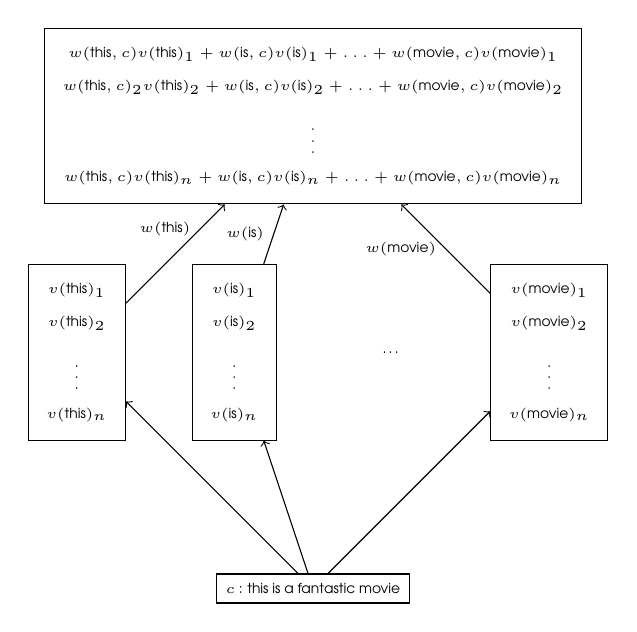
\begin{tikzpicture}
      \node[rectangle, draw] (text) at (0, 0) { \tiny $c$ : this is a fantastic movie};
    
      \matrix (v1) [draw, every node/.style={outer sep=0}, matrix of nodes, nodes in empty cells, execute at empty cell=\node{\strut}] at (-3, 3){
       \tiny $v(\textnormal{this})_1$ \\ \tiny $v(\textnormal{this})_2$ \\ \tiny \vdots \\ \tiny $v(\textnormal{this})_n$\\
      };
      \matrix (v2) [draw, every node/.style={outer sep=0}, matrix of nodes, nodes in empty cells, execute at empty cell=\node{\strut}] at (-1, 3){
        \tiny $v(\textnormal{is})_1$ \\ \tiny $v(\textnormal{is})_2$ \\ \tiny \vdots \\ \tiny $v(\textnormal{is})_n$\\
      };
      \node at (1, 3) {\tiny \dots};
      \matrix (v3) [draw, every node/.style={outer sep=0}, matrix of nodes, nodes in empty cells, execute at empty cell=\node{\strut}] at (3, 3){
        \tiny $v(\textnormal{movie})_1$ \\ \tiny $v(\textnormal{movie})_2$ \\ \tiny \vdots \\ \tiny $v(\textnormal{movie})_n$\\
    };
      \path (text) edge[->] (v1);
      \path (text) edge[->] (v2);
      \path (text) edge[->] (v3);
      \matrix (sum) [draw, every node/.style={outer sep=0}, matrix of nodes, nodes in empty cells, execute at empty cell=\node{\strut}] at (0, 6){
        \tiny $w(\textnormal{this}, c)v(\textnormal{this})_1 + w(\textnormal{is}, c)v(\textnormal{is})_1 + \dots + w(\textnormal{movie}, c)v(\textnormal{movie})_1$  \\ \tiny $w(\textnormal{this}, c)_2v(\textnormal{this})_2 + w(\textnormal{is}, c)v(\textnormal{is})_2 + \dots + w(\textnormal{movie}, c)v(\textnormal{movie})_2$  \\ \tiny \vdots \\ \tiny $w(\textnormal{this}, c)v(\textnormal{this})_n + w(\textnormal{is}, c)v(\textnormal{is})_n + \dots + w(\textnormal{movie}, c)v(\textnormal{movie})_n$ \\
      };
      \path (v1) edge[->] node[near end, left] {\tiny $w(\textnormal{this})$} (sum);
      \path (v2) edge[->] node[midway, left] {\tiny $w(\textnormal{is})$} (sum);
      \path (v3) edge[->] node[midway, left] {\tiny $w(\textnormal{movie})$} (sum);   
    \end{tikzpicture}
  \end{center}
\end{document}
